\documentclass[12pt]{article}

\usepackage[a4paper,margin=2cm,top=2cm,bottom=2cm,xetex]{geometry}
\usepackage[utf8]{inputenc}
\usepackage{color,xcolor}
\usepackage{enumitem}
\usepackage{amssymb}
\usepackage{amsthm}
\usepackage{amsfonts}
\usepackage{mathtools}
\usepackage{flexisym}
\usepackage{algorithm}
\usepackage{algorithmic}
\usepackage{tabularx}
\usepackage{xepersian}
\usepackage{amsmath}
\usepackage{physics}
\usepackage{comment}
%\usepackage{mathtools}

\DeclareFontFamily{U}{matha}{\hyphenchar\font45}
\DeclareFontShape{U}{matha}{m}{n}{ <-6> matha5 <6-7> matha6 <7-8>
matha7 <8-9> matha8 <9-10> matha9 <10-12> matha10 <12-> matha12 }{}
%\DeclareSymbolFont{matha}{U}{matha}{m}{n}
%
%\DeclareMathSymbol{\nvartrianglelefteq}{\mathrel}{matha}{"9E}
%\DeclareMathSymbol{\vartrianglelefteq}{\mathrel}{matha}{"9C}

\newcount\HWcnt
\def\ttmp#1#2#3#4#5#6#7#8#9|{\def\Wjob{#9}}%
\expandafter\ttmp\jobname |
\def\ttmp#1#2#3{\global\HWcnt=#2#3}
\expandafter\ttmp\Wjob

\settextfont[Scale = 1.0 ,
             BoldFont = *Bd ,
             ItalicFont = *It ,
             BoldItalicFont = *BdIt ,
             Extension = .ttf
            ]{XB Niloofar}
\ExplSyntaxOn
\cs_set_eq:NN
\etex_iffontchar:D
\tex_iffontchar:D
\cs_undefine:N \c_one
\int_const:Nn \c_one { 1 }
\ExplSyntaxOff
\setdigitfont[Scale = 1.0 ,
             BoldFont = *Bd ,
             ItalicFont = *It ,
             BoldItalicFont = *BdIt ,
             Extension = .ttf
            ]{XB Niloofar}
\renewcommand{\baselinestretch}{1.2}
\pagestyle{empty}

\makeatletter
\def\abj@num@i#1{%
    \ifcase #1\or الف\or ب\or ج\or د\or ه\or و\or ز\or ح\or ط\fi \ifnum #1=\z@ \abjad@zero \fi
}
\renewcommand{\theenumi}{\abjad{enumi}}
\renewcommand{\labelenumi}{\theenumi)}
\long\def\makeHead#1{%
	\begin{center}\large
		\begin{tabular}{@{}p{.33\linewidth}<{\hfill}@{}>{\hfil}p{.33\textwidth}<{}@{}>{\hfill}p{.33\textwidth}@{}}
            \textbf{محاسبات عددی} & & \textbf{سری شمارهٔ ۱} \\[.5ex]
            \textbf{نیم‌سال اول ۱۴۰۲-۱۴۰۳} & &  \textbf{موعد تحویل: #1}\\[.5ex] \hline\hline
		\end{tabular}
	\end{center}\smallskip
%	\def\theenumii{\arabic{enumii}}\def\theenumi{\alph{enumii}}\def\labelenumi{\theenumi)}\def\labelenumii{\theenumii)}%
}

\newcommand{\Rule}{\ \hfill\rule{\linewidth}{0.5pt}\hfill\ \par\vspace*{-2ex}\par}
\newcommand{\DescRule}{\ \hfill\rule{\linewidth}{1pt}\hfill\ \vspace*{-2ex}\par}
\def\rank{\mathop{\mathrm{rank}}\nolimits}

\begin{document}
\makeHead{۸ آبان}
\begin{description}
% 	\item{\textbf{سوال 1.}} \input{\jobname-q1.tex}
	
% 	\Rule
    
    \item {\textbf{سوال ۱.}}
    دستگاه غیرخطی زیر را حل کنید. (جواب را تا ۷ رقم اعشار بدست آورید)
\begin{center}
$
    \begin{cases}
    x^2 - 10x + y^2 = -8 \\
    xy^2 + x - 10y = -8
    \end{cases}
$
\end{center}
\textcolor{blue}{
حل
\\
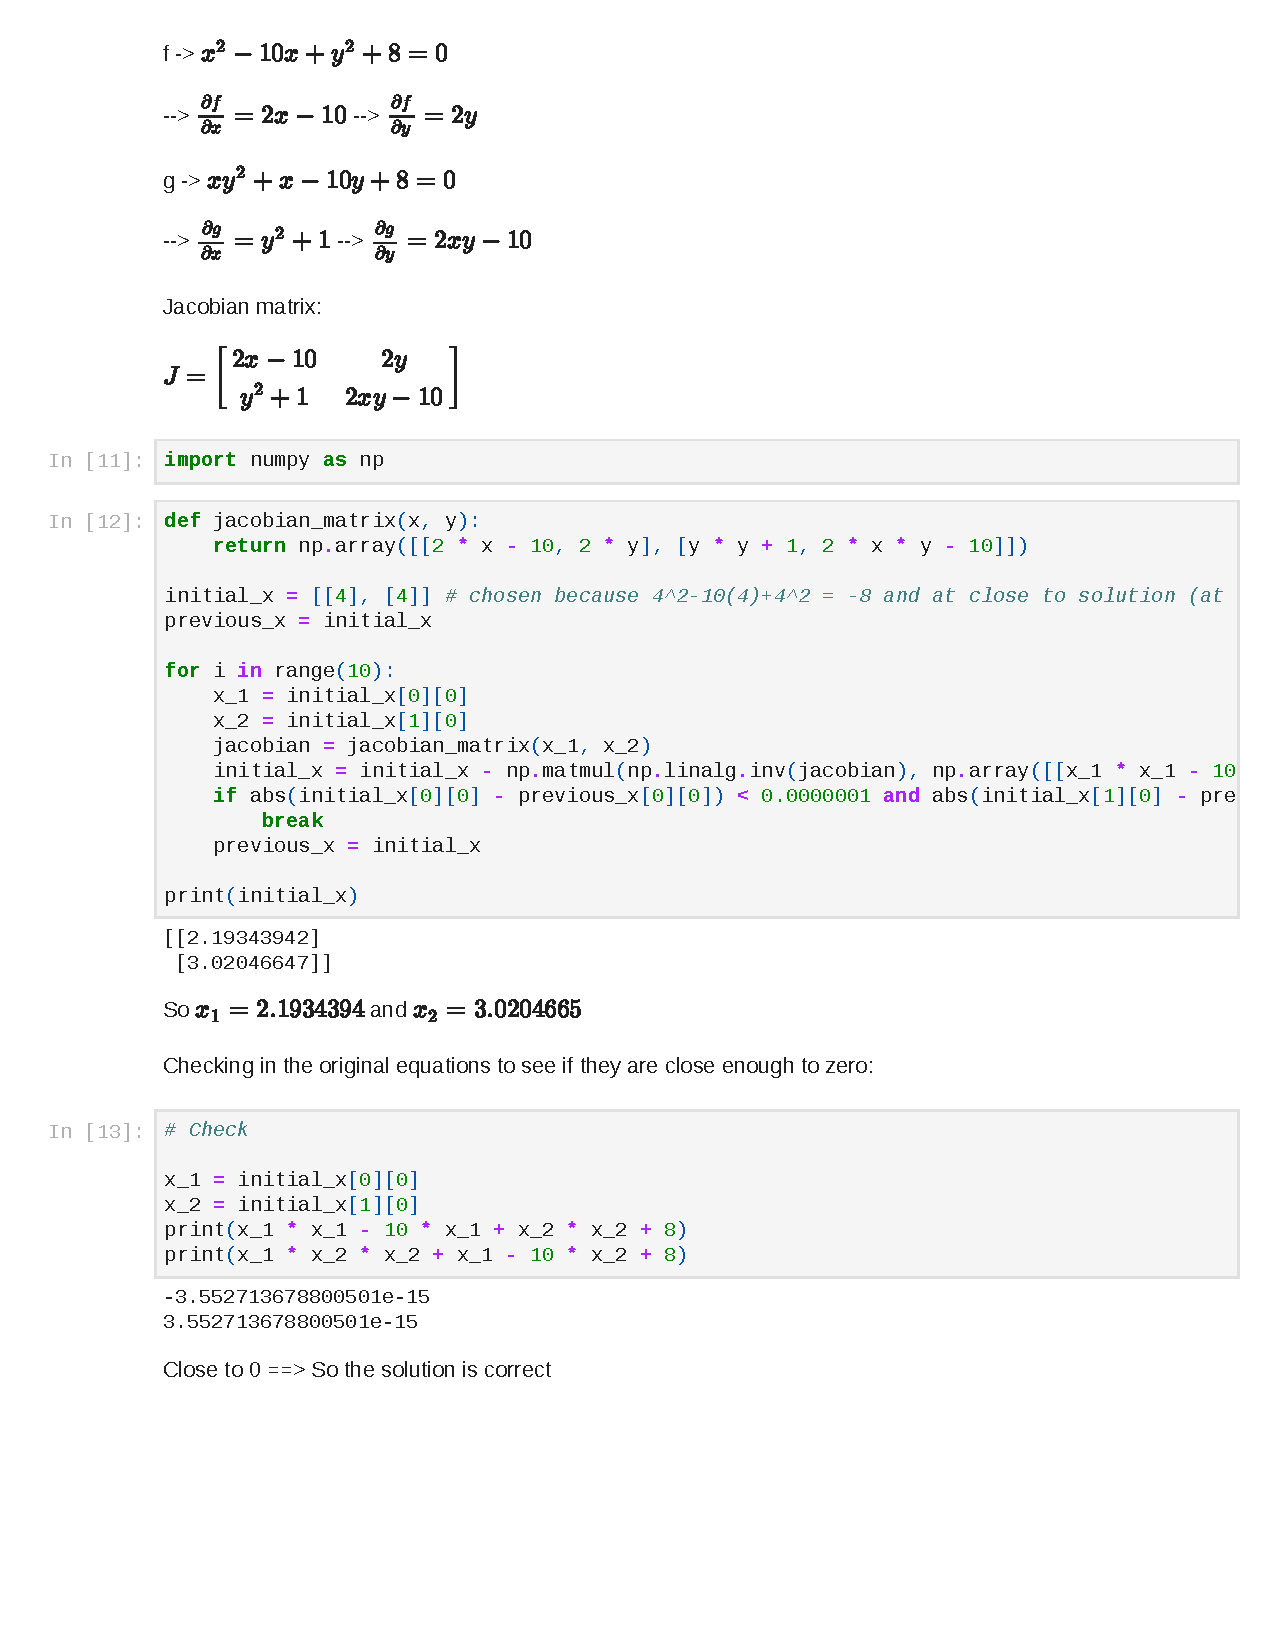
\includepdf[pages={1-},scale=1]{q9.pdf}
}
	
    \Rule

    \item {\textbf{سوال ۲.}}
    فرض کنید می‌خواهیم تابع 
$f(x)$
را با استفاده از سری مک‌لورن توابع $sin(x)$، $cos(x)$ و $tan^{-1}(x)$ روی بازه‌ی $[\frac{\pi}{2}, \frac{5\pi}{6}]$ حساب کنیم.
محاسبه کنید که هر کدام از این سه سری را حداقل باید تا چه مرتبه ای بسط دهیم تا خطایِ کلِ محاسبه‌یِ مقدارِ تابع روی کل بازه، از $10^{-5}$ کمتر شود.

$$f(x) = \frac{ 4sin^2(x) - cos(x) }{3tan^{-1}(\frac{2x}{\pi \sqrt{3}})}$$

\begin{comment}
\end{comment}
پاسخ:

ابتدا تابع k را به صورت زیر تعریف می‌کنیم:
$$k(a,b,c) = \frac{4a^2 - b}{3c}$$
حال مشاهده می‌کنیم که 
$$f(x) = k(sin(x), cos(x), tan^{-1}(\frac{2x}{\pi \sqrt{3}}))$$
حال با استفاده از فرمول خطای چند متغیر داریم:
$$\Delta k = \frac{\partial k}{\partial a} \Delta a + \frac{\partial k}{\partial b} \Delta b + \frac{\partial k}{\partial c} \Delta c$$

$$\frac{\partial k}{\partial a} = \frac{8a}{3c}$$
$$\frac{\partial k}{\partial b} = \frac{-b}{3c}$$
$$\frac{\partial k}{\partial c} = \frac{-4a + b}{3c^2}$$

حال حد بالایی برای مقادیر ماکسیمم این ضریب خطاها را روی بازه‌ی داده شده می‌یابیم:
برای سادگی ماکسیمم سینوس و کسینوس را ۱ درنظر می‌گیریم. همچنین دقت می‌کنیم که تابع وارون تانژانت صعودی است پس مقدار کمینه آن روی بازه، در نقطه $x=\pi/2$ اتفاق می‌افتد.

$$\abs{\frac{\partial k}{\partial a}} \leq \frac{8}{3 (\frac{\pi}{6})}$$
$$\abs{\frac{\partial k}{\partial b}} \leq \frac{1}{3 (\frac{\pi}{6})}$$
$$\abs{\frac{\partial k}{\partial c}} \leq \frac{5}{3 (\frac{\pi}{6})^2}$$

حال داریم:

$$|\Delta k| \leq \abs{\frac{\partial k}{\partial a} \Delta a} + \abs{\frac{\partial k}{\partial b} \Delta b} + \abs{\frac{\partial k}{\partial c} \Delta c}$$

$$|\Delta k| \leq \abs{ \frac{8}{3 (\frac{\pi}{6})} \Delta a} + \abs{\frac{1}{3 (\frac{\pi}{6})} \Delta b} + \abs{\frac{5}{3 (\frac{\pi}{6})^2} \Delta c}$$

حال داریم:

$$\frac{8}{3 (\frac{\pi}{6})} \approx 5.092$$
$$\frac{1}{3 (\frac{\pi}{6})} \approx 0.636$$
$$\frac{5}{3 (\frac{\pi}{6})^2} \approx 6.079$$

و میبینیم که 

$$10^{-2} \times 5.092 + 10^{-1} \times 0.636 + 10^{-1} \times 6.079 \approx 1$$

درواقع برای اینکه تضمین کنیم که خطای کل عبارت از $10^{-5}$ کمتر است. باید حتما خطای هر سه جمله کمتر از $10^{-6}$ باشد. اما خطای یکی از جملات باید کمتر از $10^{-7}$ باشد.

در حقیقت هر ترکیبی از خطاها که معادله زیر را ارضا کند می‌تواند جواب مساله باشد و بسته به توان محاسبانی می‌توانیم هر کدام را انتخاب کنیم.

$$5.092 \Delta a + 0.636 \Delta b + 6.079 \Delta c  \leq 10^{-5}$$

برای مثال حالت زیر را انتخاب می‌کنیم.
$$\Delta a  = 10^{-7}$$
$$\Delta b = 10^{-6}$$
$$\Delta c = 10^{-6}$$

و با استفاده از حد بالای خطای سری هر کدام تعداد جملات مورد نیاز را حساب می‌کنیم:

برای sin(.) :
$$|\Delta sin(x)| \leq \abs{\frac{x^{2n+1}}{(2n+1)!}} \leq 10^{-7}$$
$$\frac{(\frac{5\pi}{6})^{2n+1}}{(\frac{2n+1}{e})^{2n+1}} \leq 10^{-7}$$
$$(\frac{5e\pi}{6(2n+1)})^{2n+1} \leq 10^{-7}$$
$$n=9 \Rightarrow (\frac{5 \times 8.54}{6 \times 19})^{19} < (\frac{2}{5})^{19} < 10^{-7}$$

برای cos(.) : 
$$|\Delta cos(x)| \leq \abs{\frac{x^{2n}}{(2n)!}} \leq 10^{-6}$$
$$\frac{(\frac{5\pi}{6})^{2n}}{(\frac{2n}{e})^{2n}} \leq 10^{-6}$$
$$(\frac{5e\pi}{2n})^{6(2n)} \leq 10^{-6}$$
$$n=9 \Rightarrow (\frac{5 \times 8.54}{6 \times 18})^{18} < (\frac{2}{5})^{18} < 10^{-6}$$

برای $tan^{-1}(.)$ :
$$|\Delta tan^{-1}(\frac{2x}{\pi \sqrt{3}})| \leq \abs{\frac{(\frac{5}{3\sqrt{3}})^{2n+3}}{(2n+3)}} \leq 10^{-6}$$
$$\frac{(0.962)^{2n+3}}{2n+3} \leq 10^{-6}$$
با لگاریتم گیری بدست می‌آید
$$n=108$$

به دلیل عدم وجود فاکتوریل در مخرج جملات این سری، سری بسیار کند همگرا می‌شود. این کندی در تعداد عبارات مورد نیاز برای بدست آوردن دقت مورد نیاز کاملا مشهود است.



    \Rule
    
    \item {\textbf{سوال ۳.}}
    بسط تیلور تابع زیر را تا چه مرتبه ای حساب کنیم که خطای محاسبه در $x= \frac{\pi}{3}$ کمتر از $10^{-5}$ شود؟
$$f(x) = \frac{sin(x)}{x}$$

پاسخ:

راه مستقیم و قابل قبول این است که مرتبا مشتق تابع را در یک نقطه غیر صفر حساب کنیم و بسط تیلور و خطای آن را حساب کنیم.
راه ساده تر این است که از بسط مک‌لورن تابع سینوس استفاده کنیم:

$$sin(x) = \sum_{k=0}^{\infty} (-1)^k \frac{x^{2k+1}}{(2k+1)!}$$
$$\frac{sin(x)}{x} = \sum_{k=0}^{\infty} (-1)^k \frac{x^{2k}}{(2k+1)!}$$

حال با توجه به اینکه سری داده شده alternating است و قدر مطلق هر جمله آن کمتر از جمله قبل است و در حد بینهایت k تمام جملات به صفر میل میکنند (سرعت رشد مخرج به صورت فاکتوریل و سرعت رشد صورت به صورت نمایی است) پس خطای قطع سری در هر k از جمله بعدی کمتر است. به عبارت دیگر:

$$\abs{\frac{sin(x)}{x} - \sum_{k=0}^{n} (-1)^k \frac{x^{2k}}{(2k+1)!}} \leq \abs{\frac{x^{2k+2}}{(2k+3)!}}$$

$$\frac{(\frac{\pi}{3})^{2n+2}}{(\frac{2n+3}{e})^{2n+3}} \leq 10^{-5}$$
$$\frac{e}{2n+3} (\frac{e\pi}{3(2n+3)})^{2n+2} \leq 10^{-5}$$
$$n = 4 \Rightarrow \frac{2.7}{11} (\frac{8.54}{33})^{10} \leq 10^{-5}$$


    \Rule

    \item {\textbf{سوال ۴.}}
    می‌دانیم که فرمول کلی سری مکلورن به شکل 

$$\frac{1}{1 + x} = 1  - x + x^{2} - x^{3} + ...$$

می‌باشد. بنابراین، سری مکلورن $\frac{1}{2 + x}$ را پیدا کنید.

\begin{comment}
\end{comment}
پاسخ:


    $$\frac{1}{2 + x} = \frac{1}{2 (1 + \frac{x}{2})}$$
    $$= 2 (1 - \frac{x}{2} + \frac{x^{2}}{4} - \frac{x^{3}}{8}) + ...$$





    \Rule

    \item {\textbf{سوال ۵.}}
    \subsection*{الف}

برای یک تابع پیوسته و مشتق‌پذیر \( f \)، با استفاده از فرمول‌های تقریب مرکزی، معادله زیر را نشان دهید:

\[ f'(x) \approx \frac{-f(x + 2h) + 4f(x + h) - 3f(x)}{2h} \]

و بررسی کنید که خطای تقریب از مرتبه \( O(h^2) \) است.

\subsection*{ب}

با توجه به توسعه سری تیلور برای تابع کوسینوس، تایید کنید:

\[ \cos(h) + \frac{1}{2} h^2 \approx 1 \]

و نشان دهید که این تقریب یک خطای از مرتبه \( O(h^4) \) دارد.

\begin{comment}
\end{comment}
پاسخ:


    \subsection*{الف}
    از بسط تیلور حول نقطه‌ی $x$ استفاده می‌کنیم:
    
    $$f(x + h ) = f(x) + \frac{x + h - x}{1!}f'(x) + \frac{(x + h - x)^{2}}{2!}f''(x) + \frac{(x + h - x)^{3}}{3!}f^{3}(x) + ...$$
    
    $$= f(x) + \frac{h}{1!}f'(x) + \frac{h^{2}}{2!}f''(x) + \frac{h^{3}}{3!}f^{3}(x) + ... $$
    
    می‌دانیم: 
    
    $$\frac{h^{3}}{3!}f^{3}(x) + ... = O(h^{3})$$
    
    در نتیجه:
    
    $$f(x + h) = f(x) + hf'(x) + \frac{h^{2}}{2}f''(x) + O(h^{3}),  (1)$$
    
    اگر همین کار را برای $f(x + 2h)$ انجام دهیم داریم:
    
    
    $$f(x + 2h) = f(x) + 2hf'(x) + 2h^{2}f''(x) + O(h^{3}), (2)$$
    
    حال از دو معادله ۱ و ۲ می‌توان نوشت:
    
    $$\frac{4(f(x) + hf'(x) + \frac{h^{2}}{2}f''(x)) + O(h^{3})}{2h} + \frac{-(f(x) + 2hf'(x) + 2h^{2}f''(x)) + O(h^{3})}{2h} - \frac{3f(x)}{2h}$$
    
    
    $$= \frac{2hf'(x) + 3O(h^{3})}{2h} = f'(x) + O(h^{2})$$
    
    
    $$f'(x) + O(h^{2}) = \frac{-f(x + 2h) + 4f(x + h) - 3f(x)}{2h}$$
    
    
    \subsection*{ب}
    در این قسمت از بسط مکلورن استفاده می‌کنیم:
    
    $$cos(h) = 1 - \frac{h^{2}}{2!} + \frac{h^{4}}{4!} - \frac{h^{6}}{6!} + ...$$
    $$cos(h) + \frac{h^{2}}{2!} = 1 + O(h^{4})$$





    \Rule

    \item {\textbf{سوال ۶.}}
    فرض کنید یک جدول باید برای تابع 
\(f (x) = e^{x}\)
آماده شود، برای حالتی که 
\(x\)
در بازه [1, 0] است. 
فرض کنید تعداد اعشاراتی که باید برای هر ورودی آمده باشد، 
\(d \geq 8\)
است، یعنی هر مقدار حداقل به هشت رقم اعشار نمایش داده می‌شود.
همچنین تفاوت بین مقادیر 
\(x\)
مجاور، یعنی اندازه گام، 
\(h\)
است. اندازه گام 
\(h\)
چقدر باید باشد تا تضمین شود که درون‌یابی خطی، خطای مطلق حداکثر 
\(10^{-6}\)
برای همه مقادیر
\(x\)
در بازه [1, 0] دارد؟

\begin{comment}
\end{comment}
پاسخ:


    قرار دهید 
    $x_{0}, x_{1}, ...$
    نقاطی که در 
    $f$
    در آن محاسبه شده است.
    همچنین  $0 \leq x \leq 1 $
    و فرض کنید 
    $x_{j} \leq x \leq x_{j + 1} $.
    معادله زیر نشان می‌دهد که خطا در درون‌یابی خطی برابر است با:

    $$\abs{f(x) - P(x)} = \abs{\frac{f^{(2)}(\xi)}{2!}(x - x_{j})(x - x_{j+1})} = \frac{\abs{f^{(2)}(\xi)}}{2} \abs{(x - x_{j})}\abs{(x - x_{j+1})}$$

    که گام حرکت برابر است با h
    ،بنابراین $x_{j} = jh, x_{j + 1} = (j + 1)h$
    و 

    $$\abs{f(x) - P(x)} \leq \frac{\abs{f^{(2)}(\xi)}}{2} \abs{(x - jh)(x - (j + 1)h)}$$

    بنابراین

    $$\abs{f(x) - P(x)} \leq \frac{\max_{\xi \in [0, 1]} e^{\xi}}{2} \max_{x_{j} \leq x \leq x_{j + 1}} \abs{(x - jh)(x - (j + 1)h)} \leq \frac{e}{2} \max_{x_{j} \leq x \leq x_{j + 1}} \abs{(x - jh)(x - (j + 1)h)}$$

    تابع 
    $g(x) = (x - jh) (x - (j + 1)h)$
    را برای $jh \leq x \leq (j + 1)h$
    در نظر بگیرید.  چون

    $$g'(x) = (x - (j + 1)h) + (x - jh) = 2 (x - jh - \frac{h}{2}),$$

    نقطه‌ی اکسترمم تابع g برابر است با $x = jh + \frac{h}{2}$ و $g(jh + \frac{h}{2}) = \frac{h^{2}}{4}$.

    از آنجایی که $g(jh) = 0, g((j + 1)h) = 0$ حداکثر مقدار $\abs{g'(x)}$  در بازه‌ی  $[jh, (j + 1)h]$ در نقطه‌ی اکسترمم باید باشد که نشان می‌دهد: 

    $$\abs{f(x) - P(x)} \leq \frac{e}{2} \max_{x_{j} \leq x \leq x_{x + 1}} \abs{g(x)} \leq \frac{e}{2}.\frac{h^{2}}{4} = \frac{eh^{2}}{8}$$.

    حال داریم:

    $$\frac{eh^{2}}{8} \leq 10^{-6}$$
    $$ h < 1.72 \times 10 ^ {-3}$$

    در نهایت چون $n = \frac{(1 - 0)}{h}$ باید یک عدد صحیح باشد، یک گزینه‌ی قابل‌قبول طول گام می‌تواند $h = 0.001$ باشد.


    \Rule

	\vspace*{-2ex}\ \hfill\textbf{موفق باشید.}
\end{description}
\end{document}